\documentclass[preprint,12pt, a4paper]{elsarticle}

\usepackage{amssymb}
\usepackage{float}
\usepackage{listings}
\usepackage{hyperref}
\usepackage{xcolor}
\setlength{\parindent}{0pt}
\lstdefinestyle{mystyle}{
    basicstyle        = \ttfamily\footnotesize,
    breakatwhitespace = false,
    breaklines        = true,
    captionpos        = b,
    keepspaces        = true,
    numbersep         = 5pt,
    showspaces        = false,
    showstringspaces  = false,
    showtabs          = false,
    keywordstyle      = \color{blue},
    stringstyle       = \color{green},
    commentstyle      = \color{red}\ttfamily
}

\lstset{style=mystyle}

\restylefloat{table}
\journal{SoftwareX}

\begin{document}
\renewcommand{\labelenumii}{\arabic{enumi}.\arabic{enumii}}

\begin{frontmatter}
\title{omnisolver-bruteforce: a distributed GPU exhaustive solver plugin update for Omnisolver\tnoteref{refers}}
\tnotetext[refers]{Refers to the previous Omnisolver publication~\cite{jalowiecki2021omnisolver}.}

\author[1]{Konrad Ja\l{}owiecki}
\author[1]{{\L}ukasz Pawela}
\author[1]{Bart{\l}omiej Gardas}
\author[1]{Jan Tuziemski}

\address[1]{Institute of Theoretical and Applied Informatics, Polish Academy of
Sciences, Ba{\l}tycka 5, 44-100 Gliwice, Poland}

\begin{abstract}
This manuscript reports a software update in the Omnisolver ecosystem introduced
in~\cite{jalowiecki2021omnisolver}. We present \texttt{omnisolver-bruteforce}, a
dedicated Omnisolver plugin providing exact exhaustive search for QUBO and Ising
instances on CUDA-enabled GPUs, including distributed execution with Ray. The
update addresses the main practical limitation of the fast ground-state path:
numerical instability for larger instances (\(N \geq 40\)) when energies are
tracked through long chains of incremental updates. In the release-candidate
code branch \texttt{lp/recompute-energy}, we stabilize this path with periodic
exact energy recomputation (re-anchoring), compensated subtraction in the
incremental updates, and refresh of best-state buffers after re-anchoring. The
public sampler API remains unchanged. The updated implementation keeps the
distributed exhaustive-search capability and solves a dense \(N=60\) instance in
around three days on eight NVIDIA H100 GPUs.
\end{abstract}

\begin{keyword}
QUBO \sep spin--glass \sep discrete optimization \sep exhaustive search \sep
Omnisolver plugin \sep software update
\end{keyword}

\end{frontmatter}

\section*{Metadata}
\label{}

\begin{table}[!h]
\begin{tabular}{|l|p{6.2cm}|p{6.8cm}|}
\hline
\textbf{Nr.} & \textbf{Code metadata description} & \textbf{Value} \\
\hline
C1 & Current code version & \texttt{0.0.4-1-g71d521d} (release-candidate branch
\texttt{lp/recompute-energy}) \\
\hline
C2 & Permanent link to code/repository used for this code version &
\url{https://github.com/euro-hpc-pl/omnisolver-bruteforce/tree/71d521dca8a0207267cff56d343b1f3ffcbf05b2}
\\
\hline
C3 & Permanent link to reproducible capsule (if available) & Not available for this version. \\
\hline
C4 & Legal Code License & Apache 2.0 \\
\hline
C5 & Code versioning system used & git \\
\hline
C6 & Software code languages, tools, and services used & Python, C++, Cython,
CUDA, Ray \\
\hline
C7 & Compilation requirements, operating environments \& dependencies & Linux,
CUDA Toolkit, \texttt{Python >= 3.10}, \texttt{omnisolver >= 0.0.4},
\texttt{dimod}, \texttt{numba}, \texttt{numpy} \\
\hline
C8 & If available Link to developer documentation/manual &
\url{https://euro-hpc-pl.github.io/omnisolver/},
\url{https://github.com/euro-hpc-pl/omnisolver-bruteforce} \\
\hline
C9 & Support email for questions & \verb|lpawela@iitis.pl|\\
\hline
\end{tabular}
\caption{Code metadata}
\label{codeMetadata}
\end{table}

\section{Motivation and significance}

Omnisolver provides a unified framework for binary quadratic model solvers,
including shared command-line and input/output
interfaces~\cite{jalowiecki2021omnisolver}. This paper is not a new submission
of that framework; it is a software update paper introducing and documenting one
specific solver plugin: \texttt{omnisolver-bruteforce}.

The role of this plugin is to provide exact reference solutions for QUBO and
Ising instances. Such exact solutions are essential when benchmarking
approximate methods and when verifying results produced by NISQ-oriented
workflows~\cite{preskill2018quantum}. The exhaustive-search approach guarantees
optimality, but practical performance depends on careful GPU implementation and
distributed orchestration.

Before this update, the main limitation in the fast ground-state mode was
numeric drift for larger instances (\(N \geq 40\)). That mode uses incremental
energy updates along Gray-code trajectories; for long trajectories in
\texttt{float32}, rounding errors may accumulate and degrade energy accuracy.
The release-candidate branch \texttt{lp/recompute-energy} addresses this issue
while preserving the existing API and distributed scaling model.

The key update contributions are:
\begin{itemize}
    \item Numerical stabilization of the \texttt{num\_states=1} GPU path via
    compensated updates and periodic exact energy recomputation.
    \item Synchronization of best-state buffers with recomputed energies to keep
    candidate minima consistent.
    \item Guardrails in kernel-step logic and 64-bit-safe bit operations for
    large-state enumeration.
    \item Extended GPU tests validating energy correctness against exact
    recomputation and \texttt{dimod.ExactSolver} on representative instances.
\end{itemize}

\section{Software description}\label{sec:software-desc}

\subsection{Software architecture}
The plugin exposes two sampler classes:
\begin{itemize}
    \item \texttt{BruteforceGPUSampler}: single-node GPU exhaustive search.
    \item \texttt{DistributedBruteforceGPUSampler}: distributed exhaustive
    search over multiple GPUs and/or hosts via
    Ray~\cite{DBLP:journals/corr/abs-1712-05889}.
\end{itemize}

Performance-critical kernels are implemented in CUDA/C++, and exposed to Python
through a Cython wrapper. The plugin follows Omnisolver's plugin mechanism, so
users can call it from Python or from Omnisolver's CLI without custom glue code.

For distributed runs, the solver fixes \texttt{num\_fixed\_vars} variables and
enumerates all \(2^k\) fixed assignments. Each assignment defines a subproblem
with \(N-k\) unfixed variables solved by the GPU sampler. Ray schedules
subproblems across workers; partial results are gathered and merged on the
controller node. The workflow is shown in Fig.~\ref{fig:arch}.

\begin{figure}
    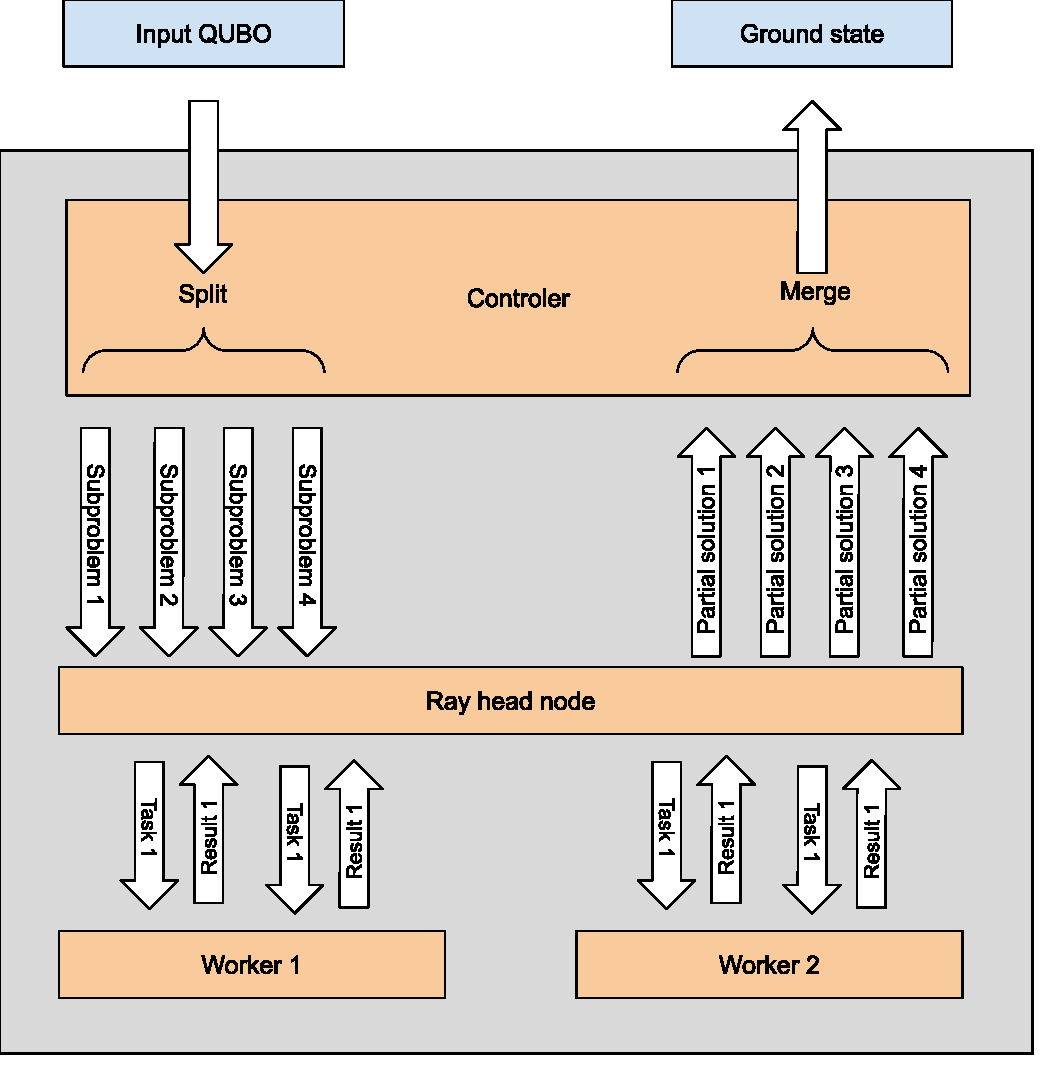
\includegraphics[width=\textwidth]{figs/omnisolver-distributed-diagram.pdf}
    \caption{ Distributed execution of \texttt{omnisolver-bruteforce}. The input
        BQM is partitioned into fixed-variable subproblems, dispatched to Ray
        workers, solved by GPU samplers, and merged into the final low-energy
        result. }
    \label{fig:arch}
\end{figure}

\subsection{Update-specific algorithmic changes}
The update focuses on the ground-only fast path (\texttt{num\_states=1}) in the
GPU backend. The previous implementation relied solely on incremental energy
differences along Gray-code steps. For \(N \geq 40\) in \texttt{float32}, this
could accumulate numerical error.

The updated backend introduces three stabilization mechanisms:
\begin{itemize}
    \item \textbf{Compensated subtraction} during incremental updates to reduce
    cancellation error.
    \item \textbf{Periodic re-anchoring}, i.e., recomputing exact energies from
    states at controlled intervals.
    \item \textbf{Best-buffer refresh} after re-anchoring, ensuring tracked
    minima remain consistent with recomputed energies.
\end{itemize}

In this branch, stabilization is automatically enabled for the large-\(N\)
\texttt{float32} ground-only configuration: \texttt{num\_states=1},
\texttt{dtype=float32}, \(N \geq 40\). No public method signature changed in
this update.

\subsection{Software functionalities}
Major plugin functionalities are:
\begin{itemize}
    \item exact exhaustive search for BINARY and SPIN BQMs (with internal
    vartype conversion),
    \item low-energy-spectrum mode (\texttt{num\_states>1}) and optimized
    ground-state mode (\texttt{num\_states=1}),
    \item distributed decomposition with Ray through \texttt{num\_fixed\_vars},
    \item Python API and Omnisolver CLI integration as the
    \texttt{bruteforce-gpu} solver,
    \item \texttt{dimod.SampleSet} output with runtime metadata (\texttt{solve\_time\_in\_seconds}).
\end{itemize}

\subsection{Validation in the update branch}
The update branch includes additional GPU tests for correctness of the
stabilized path. They verify that returned energies are consistent with CPU-side
exact energy evaluation and that ground-state results agree with
\texttt{dimod.ExactSolver} on tractable small instances. An opt-in performance
guard test is also included to ensure the stabilization path remains practical
in representative workloads.

\section{Illustrative examples}
The package is distributed as \texttt{omnisolver-bruteforce} on PyPI and can be
used standalone or through Omnisolver. Listing~\ref{lst:bf-code} shows an
example script that generates random instances and runs the distributed solver.

\lstinputlisting[
language=Python,
caption={Example distributed benchmark script for \texttt{omnisolver-bruteforce}},
label={lst:bf-code}
]{code/bf.py}

Example Ray startup commands for an 8-GPU, two-node setup (4 GPUs per node) are:

\begin{lstlisting}[language=bash,caption={Example Ray commands for distributed execution},label={lst:ray-commands}]
# Head node
ray stop --force
ray start --head --port=6379 --num-gpus=4

# Worker node
ray stop --force
ray start --address='<HEAD_NODE_IP>:6379' --num-gpus=4

# Run benchmark script from the project root
python code/bf.py --start 60 --stop 40 --step -2 --skip-existing
\end{lstlisting}

Representative runtime results of this distributed workflow are shown in
Fig.~\ref{fig:runtimes}.

\begin{figure}
\centering

\includegraphics[width=\textwidth]{distributed.pdf}
\caption{Runtime of the distributed \texttt{omnisolver-bruteforce} solver as a function of problem size.}
\label{fig:runtimes}
\end{figure}

\section{Impact}
This update contributes a production-ready exhaustive solver plugin inside the
Omnisolver ecosystem. It combines exactness guarantees with distributed GPU
execution, making it useful as a certification and benchmarking backend for
QUBO/Ising research pipelines.

The key practical outcome is that the previously observed instability region for
large-\(N\) fast ground-state runs is addressed in the release-candidate branch.
This substantially improves reliability of exact-energy reporting in the regime
where exhaustive verification is most computationally expensive.

The solver retains the previously demonstrated large-instance capability: a
dense \(N=60\) instance can be solved in around three days on \(8\times\) NVIDIA
H100 GPUs. This makes exhaustive verification feasible for problem sizes that
are beyond the range of simple single-device brute-force baselines.

\section{Discussion and future extensions}
The update improves numerical robustness in the \texttt{num\_states=1} path,
but it does not change the exponential complexity of exhaustive search. In
practice, this solver remains most useful as a ground-truth backend for
benchmarking, debugging, and verification of approximate pipelines.

\subsection{Threats to validity}
The reported runtime envelope and numerical behavior depend on the hardware and
software stack, including GPU model, CUDA version, compiler flags, and Ray
runtime configuration. In particular, the \(N=60\) result on \(8\times\)H100
should be interpreted as a hardware-specific operating point rather than a
universal runtime guarantee.

The stabilization path is validated in this update branch using representative
test instances and exact-energy cross-checks, but pathological coefficient
distributions can still stress \texttt{float32} arithmetic. For high-risk use
cases, users should validate with additional seeds and, where feasible, compare
against \texttt{float64} or exact small-scale baselines.

\subsection{When exhaustive bruteforce is not the right tool}
This solver is not intended for routine large-scale optimization where strict
latency constraints or limited GPU resources dominate. Because exhaustive search
scales exponentially, approximate or heuristic solvers are typically a better
primary method when the objective is fast near-optimal solutions for larger
instances.

In practical workflows, \texttt{omnisolver-bruteforce} is best used as a
calibration and certification backend: to validate solver quality on selected
instances, estimate optimality gaps, and debug model encodings.

A first extension path is broader precision policy control. The current
stabilization is automatically enabled for large-\(N\) \texttt{float32}
ground-only runs. Future versions can expose explicit user controls for
re-anchoring cadence and compensated-update modes, so users can tune stability
and runtime for specific hardware and instance families.

A second extension path is distributed post-processing. The present design
gathers subproblem results and merges them on the controller node. For very
large clusters, hierarchical merge strategies or tree reductions can reduce
controller bottlenecks and improve scalability.

A third extension path is stronger reproducibility packaging. Publishing a
versioned benchmark capsule with fixed seeds, hardware descriptors, and command
presets would make cross-platform validation of both runtime and numerical
behavior easier for the community.

\section{Conclusions}
We presented \texttt{omnisolver-bruteforce} as a SoftwareX update in the
Omnisolver line of software. The update keeps the existing user API and
distributed architecture while resolving the main numerical-stability limitation
of the fast ground-only GPU path for \(N \geq 40\). As a result, the plugin
remains a practical exact solver for large QUBO/Ising benchmarking workloads,
including the \(N=60\), \(8\times\)H100 operating point.

\section{Conflict of Interest}
No conflict of interest exists. The authors confirm that there are no known
financial or personal relationships that could have appeared to influence the
work reported in this paper.

\section*{Acknowledgements}


\bibliographystyle{elsarticle-num}
\bibliography{bruteforce.bib}

\end{document}
\endinput
